\documentclass[12pt]{article}
\usepackage[T1]{fontenc}
\usepackage[utf8]{inputenc}
\usepackage[spanish]{babel}
\usepackage{graphicx}
\usepackage{float}
\usepackage[left=2.7cm,top=2.8cm,right=2.7cm,bottom=2.8cm]{geometry} 
\usepackage{url}

\title{\large Planificación de Redes \\ \huge Implementación de red Ad-hoc en ruta G-68\\}
\author{\\ \ \\ \ \\ \ \\ \ \\ \ \\
	Eduardo Barra: 2730038-3\\
	Adan Morales: 2830042-5\\
	Diego Riquelme: 2621044-5}
\date{\today}

\begin{document}
\maketitle
\newpage
\tableofcontents
\thispagestyle{empty}

\newpage
\section{Introducción}

En el presente informe se realizará la planificación de una red Ad-Hoc en una carretera, en la 
cual los automóviles que usen la norma IEEE 802.11p, podrán almacenar y retransmitir paquetes de datos. 
La carretera seleccionada será la ruta 68, que une Valparaíso y Santiago, la cual fue seleccionada por 
el importante flujo vehicular en ambos sentidos.\\

La importancia de este trabajo radica en lo difícil que es proporcionar redes de banda ancha a los 
vehículos en las carretera, ya que a la velocidad por la cual transitan y sumado a los  tamaños de las 
celdas, por consiguiente los vehículos cruzan constantemente estos límites causando una gran cantidad 
de handoff. Por otro lado, el estándar IEEE 802.11p utiliza la banda de 5,9 GHz, con lo que además la
capacidad de servicio no puede ser 
simplemente aumentando el número de dispositivos de red, ya que esto podría causar excesiva 
interferencia.\\

Por tanto y en base a lo anterior se busca un diseño óptimo, en el cual las antenas estarán distribuidas
de la mejor manera y luego al establecer la red Ad-Hoc, serán los vehículos los que se utilizarán para 
el reenvío de paquetes y poder establecer la comunicación desde un nodo (vehículo) a la red interna o 
externa.\\

Luego la red traerá beneficios a los usuarios, como, conexión a Internet, revisar correo, navegar por 
páginas web, acceso a mapas on-line, localización y aplicaciones, etc.\\

A continuación en la figura 1 se muestra un bosquejo de la red.
\begin{figure}[H]
  \centering
      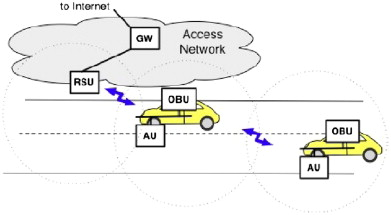
\includegraphics[width=0.6\textwidth]{img1}
	    \caption{Elementos principales de la red.}
	\label{fig:adhoc}
\end{figure}
\footnotesize
GW - Puerta de enlace, dará la conexión a internet.

OBU (On-Board unit) - Es la unidad o dispositivo que estará a bordo de los vehículos para poder realizar 
la red ad-hoc.

RSU (Road-Side Unit) - Son las antenas que proporcionarán la señal para que los vehículos puedan comunicarse 
con el exterior.

\normalsize
\newpage
\section{Método de estimación de la demanda del tráfico.}

La estimación de tráfico se realiza en base a la calidad del servicio que se quiere brindar a cada 
usuario. El objetivo de la red es otorgar acceso a servicios básicos de comunicación de internet, tales
como revisar correo, navegar por internet, acceso a mapas on\-line. Además se quiere dejar la puerta 
abierta al desarrollo de aplicaciones relacionadas con la localización de los vehículos, ubicación de 
restaurantes, gasolineras, alarma en caso de accidentes, entre otras.

Para lo anteriormente descrito, el valor práctico máximo es de aproximadamente  1  Mbps,  y  como  
valor  mínimo  para  establecer  la comunicación se utiliza un ancho  de  banda   de  512  kbps,  por 
tanto  bajo este parámetro no será posible establecer comunicación con otro dispositivo.

\section{Método de ubicación de los nodos.}

Al ser una red ad-hoc implementada en una carretera, el tráfico que exista en esta, dependerá 
parcialmente de la cantidad de congestión vehicular que exista en la carretera, para esto se cuenta 
con los datos existentes en el paper.

Luego se calcula la densidad de tráfico existente en la ruta 68, para ello con datos del sitio 
\url{http://servicios.vialidad.cl/censo/index.htm} se extrae la cantidad promedio de vehículos en un 
tiempo de 24 horas para los periodos de verano, invierno y primavera en 2010, en donde se obtiene que 
en promedio circulan 4518 vehículos en un día, y haciendo la relación con la velocidad con que se 
realizarán los cálculos, se tiene que:\\

\begin{tabular}{ l  l }
Distrancia tramo ruta G-68: \qquad $110.21[km].$ & \footnotesize (1) \normalsize \\
\tiny  & \\ \normalsize
Velocidad promedio en la ruta: \qquad $80 [\frac{km}{hr}].$ & \footnotesize (2) \normalsize \\
\tiny & \\ \normalsize
Tiempo en ir desde Santiago a Valparaiso: $T_{Stgo-Valpo}= \frac{110,21 [km]}{80 \frac{km}{hr}}= 1.38[hr]$ &
\footnotesize (3) \normalsize \\ 
\tiny & \\ \normalsize
$X_{\frac{vehic}{día}}=$ \large $\frac{3615_{verano} + 4980_{invierno} + 4959_{primavera}}{3} = $
\normalsize $4518 [\frac{vehic}{dia}]$ & \footnotesize (4) \normalsize\\
\tiny & \\ \normalsize
Vehículos en una hora: \qquad \large $\frac{4518 [vehic]}{24 [hr]}=$\normalsize $188,25[\frac{Vehic}{hr}]$ & 
\footnotesize (5) \normalsize\\
\tiny & \\ \normalsize
Vehículos por kilómetro: \qquad \large $\frac{188.25 [\frac{vehic}{hr}]}{80 \frac{Km}{hr}} =$
\normalsize $2,35 [\frac{Vehic}{Km}]$ & \footnotesize (6) \normalsize \\
\tiny & \\ \normalsize
\end{tabular}

Para este supuesto se hace que son 2,35 vehículos en una sola dirección de la ruta, por lo tanto si se 
extrapola a que la carretera es en ambos sentidos, serían 4.7 vehículos en la carretera en un kilómetro.

Por otro lado utilizando la herramienta googlemaps, se realizan unas 20 muestras en el tramo de la ruta 
G-68, en donde se tienen que el minimo de autos en un kilómetro de la carretera es de 2 vehículos, y el 
máximo de vehículos es de 13, sin considerar los puntos en donde se producen atochamientos como son los 
puntos de peaje.

Cabe señalar que ambas muestras no son 100\% fiables, ya que en el primer caso se consideran sólo 4518 
vehículos por día, por lo que este valor no toma en cuenta que por ejemplo durante la noche hay menor 
tráfico que al medio día. Por otro lado, al usar Google Maps, no se puede precisar en qué momento del día 
fueron tomadas las fotografías. Por estas dos razones, ambos factores entregan datos sólo sirven como 
referencias para ciertos escenarios, en los cuales eventualmente sería propuesta la red.

Para este problema, se consideran tres casos:
\paragraph{Primer caso:} Solamente antenas.

En primera instancia, una de las principales problemáticas que se tienen que solucionar es encontrar la 
distancia entre las antenas. 

Según se aprecia la figura \ref{fig:s-adhoc}, la distancia máxima de cobertura por antena, es de 2 Km, sin embargo no 
se considera la red Ad-hoc, vale decir, se consideran solamente las antenas sin que los automóviles sean 
repetidores. En este caso, si se considera la distancia Valparaíso-Santiago de 110,21 km, se necesitaría 
entonces:
\large $$ \frac{110,21 [km]}{2 [\frac{km}{antena}]}= 55,156 [antenas] \qquad \tiny(7)$$ \normalsize \\

Luego, con 56 antenas se cubre la totalidad del tramo sin la necesidad de vehículos, entregando así un 
100\% de disponibilidad del sistema.

Sin embargo, a medida que se va considerando la red Ad-hoc entre los vehículos, se puede ir  ampliando 
la separación entre las antenas.  

\begin{figure}[H]
  \centering
      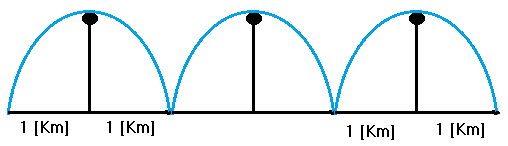
\includegraphics[width=0.6\textwidth]{s-adhoc}
	    \caption{Caso solo con antenas, sin utilizar red Ad-hoc.}
	\label{fig:s-adhoc}
\end{figure}
\paragraph{Segundo caso:} Distancia entre repetidores.

Para el cálculo de la separación de las antenas, se realizarán algunas observaciones.

Ahora el parámetro a considerar es el radio de transmisión de los dispositivos en los vehículos, cuyo 
valor es $300[m]$ para una antena de tipo omnidireccional.

Luego, es necesario considerar un espacio mínimo de espacio sin visión entre las antenas de los vehículos, 
como se muestra en la figura \ref{fig:adhoc1}
\begin{figure}[H]
  \centering
      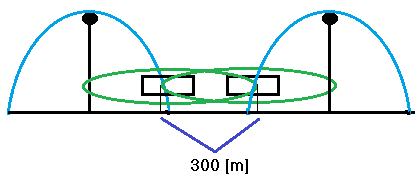
\includegraphics[width=0.5\textwidth]{adhoc1}
	    \caption{Caso sin visión directa de las antenas (NLOS).}
	\label{fig:adhoc1}
\end{figure}

Este espacio es de $300[m]$, que es la distancia para que el repetidor del vehículo pueda captar la señal. 
Se puede realizar el cálculo medio para obtener la probabilidad de que en los próximos 300 [mts] haya un 
vehículo:\\

P(en 2.35 km haya al menos 1 vehiculo) = $1$ \\            

P(en X km haya al menos 1 vehiculo) = $0.3$  \\        

\Large $\frac{2.35}{1} = \frac{X}{0.3}$ \normalsize \qquad $\Rightarrow \qquad X = 0.70$\\

Por consiguiente, la probabilidad media de que en los próximos 300 [mts] haya un automóvil es de 0.7, 
lo que se traduce en que existe un 70\% de disponibilidad en el tramo en una situación NLOS.\\
\paragraph{Tercer caso:} Separación mayor entre automóviles.
Por la ecuación (6), el valor promedio de vehículos por km es 2.35, el cual se puede considerar como 
la distancia entre vehículos. Además, el valor sigue una distribución exponencial con parámetro 
$\lambda=2,35 [\frac{veh}{km}]$. Por tanto la expresión para modelar la distribución de probabilidad queda 
de la forma:
$$ F[x]= 1-e^{-\lambda \cdot x} \qquad \tiny (8)$$

En este caso, es necesario considerar 600 [mts] de separación entre los vehículos, pero para que exista 
disponibilidad tiene que haber a lo menos un auto en un radio de 300 metros; en 600 metros por lo menos 2.
Entonces este cálculo contempla no sólo la regla de 3 anterior, si no que además la probabilidad de 
encontrar un auto separado 300 metros del otro.

Luego, los cálculos para el tercer caso se presentan a continuación:\\

P(Exista un vehículo a 300[mts]) = $1-e^{-2.35 \cdot 0.3} = 0.51$ \qquad \ \qquad (9)\\

Prob final = P(Exista un vehículo a 300 [mts] $\cdot$ 0,7) = 0.35 \qquad \ \qquad (10)

\newpage
\section{Determinación de los enlaces a instalar}
Se puede decir que la determinación de los enlaces se divide en 3 partes:

\paragraph{- Enlaces en V2V (vehicle-to-vehicle)\\}
Los enlaces propios de una red ad-hoc, en particular una Vehicular Ad-hoc Network (VANET) son 
inalámbricos y dinámicos, no son 
establecidos a priori, sino que a medida que los vehículos van avanzando en la carretera los enlaces se 
van estableciendo y dependen en gran parte al (los) protocolo(s) que se implemente(n).\\

\paragraph{- Enlaces V2I (o también V2R vehicle-to-infrastructure o vehicle-to-RoadSideUnit)\\}
El enlace que se establece entre el OBU (dispositivo montado en un vehículo) y el RSU ubicado a un 
costado de la carretera también es inalámbrico, y es creado de forma dinámica a medida que el vehículo 
pasa cerca del punto de acceso.\\

\paragraph{- Enlaces RSU a GW\\}
Los enlaces a establecer entre los Road-Side Unit y el gateway que dará el acceso a internet será por 
fibra óptica debido a que ya existirá un retardo propio en la comunicación ad-hoc, por lo tanto haciendo
los enlaces por cable UTP sería agregar aún más retardo, además por si eventualmente se decide agregar 
más servicios a la red que necesiten un mayor ancho de banda, se necesitará una comunicación más 
expedita.

En base a la geografía de la zona y según la distribución de las antenas se escoge una topología tipo 
bus. Además se busca establecer tolerancia a fallos, por lo cual se escoge una topología tipo anillo, 
en donde el enlace de fibra comenzará y terminará en un nodo central el cual será el que procesará las 
conexiones y comunicación hacia internet y dentro de la misma red.
\paragraph{Costos monetarios de los enlaces:\\}
Para la comunicación V2V, no existen costos en los enlaces ya que son inalámbricos, aunque si 
existe un costo asociado al dispositivo a instalar en los vehículos para realizar la comunicación, el 
costo de estos dispositivos bordea desde los \$12.000 a los \$60.000.

En la comunicación V2I o V2R, tampoco existe un costo asociado a los enlaces ya que serán inalámbricos, 
pero si al igual que el punto anterior, si existe un costo de adquisición de los dispositivos, 
instalación de estos y luego su posterior configuración, el precio de estos dispositivos es de unos 
\$130.000 a \$200.000 aproximadamente.

En la comunicación de los RSU al GW el precio de los enlaces sería el propio de establecer una red de 
fibra óptica, esto es, el costo de adquisición de la fibra, instalación de esta ya sea como tendido 
eléctrico por postes o subterráneo, conectores, amplificadores, multiplexores, entre otros.

\paragraph{Costos en ruteo}

La topología al ser de tipo anillo, hace que el ruteo de los paquetes sea en una dirección, por lo que 
el costo se basa en la distancia al nodo central, entonces la comunicación se realizará por el lado más 
cercano a este nodo, y el ``otro lado del anillo'' se utilizará en caso de falla a modo de redundancia.\\ 

\newpage
\section{Topología final}
La descripción de la topología se divide en 2 partes, la primera de ellas corresponde a la red de fibra 
óptica, la segunda como red inalámbrica.
\paragraph{Topología de Fibra Óptica:}
La topología de la de red de fibra, es la que se muestra a continuación en la figura \ref{fig:anillo_FO}.
\begin{figure}[H]
  \centering
      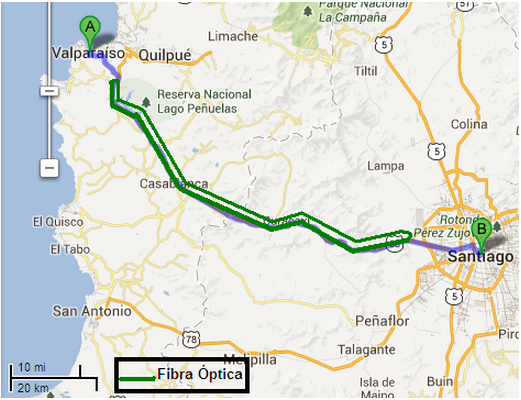
\includegraphics[width=0.7\textwidth]{anillo_FO}
	    \caption{Anillo de fibra que interconecta la red.}
	\label{fig:anillo_FO}
\end{figure}

\paragraph{Topología de Red Inalámbrica}
\paragraph{Red Wifi:} 
Se presenta como el modelo clásico de una Vehicular Ad-hoc Network (VANET), con ciertos puntos de acceso 
(RoadSide Unit), en donde ésta será la infraestructura por los cuales los vehículos equipados con un
dispositivo wireless podrán tener acceso a la red de la carretera y permitirles acceder a internet.

\paragraph{Red Ad-Hoc:}
En esta sección de la red todos los nodos (vehículos equipados con un dispositivo wireless) presentan 
funciones iguales en cuanto al enrutamiento, esto quiere decir, que en los tramo en los cuales la señal de 
los RSU no sea alcanzada por los nodos, estos comenzarán a transmitir los paquetes unos con otros de manera 
de hacerlos llegar a destino (ya sea otro nodo en particular o la siguiente RSU). Por lo tanto se considera 
una topología de tipo plana en donde no existe la necesidad de establecer jerarquía ya que cada vehículo es 
igual de importante en la red.

Cabe señalar que el enrutamiento de la red ad-hoc va a ser de tipo Flooding el cual es un proceso 
distribuido en que un nodo transmite un paquete de información a todos sus vecinos y estos a su vez 
transmiten el paquete a sus vecinos respectivos, permitiendo que el paquete se propague por toda la red. 
Este tipo de enrutamiento no requiere conocimiento sobre la topología de la red. Los paquetes se 
transmiten por broadcast a todos los destinos con la expectativa de que alcancen el nodo destino o un RSU.

\begin{figure}[H]
  \centering
      \includegraphics[width=0.7\textwidth]{}
	    \caption{Topología final superpuesta en área geográfica.}
	\label{fig:top_final}
\end{figure}

\newpage
\section{Trabajo Futuro}
Los aspectos que quedan por considerar son:\\
\paragraph{$\cdot$}Casos en que la línea de vista esté obstruida por elementos geográficos, ya que se 
consideró solamente el caso ideal en que nada se interponga entre la señal y las antenas.
\paragraph{$\cdot$}El funcionamiento acertado de las antenas. Debido a elementos naturales de la antena, 
como también a la geografía, el alcance estimado por antena no será el mismo para todas, por tanto, hay 
que considerar que ciertos tramos serán de menor alcance.
\paragraph{$\cdot$}En el trabajo, no se consideraron los túneles y peajes, ya que el primero de ellos es 
un caso especial de transmisión, mientras que en los peajes al detenerse los vehículos, se rompe el 
supuesto de velocidad promedio de $80 \frac{km}{hr}.$

\newpage
\section{Apreciación personal del trabajo realizado}

\newpage
\bibliographystyle{abbrv}
%\bibliography{main}
\section{Fuentes}
\url{http://en.wikipedia.org/wiki/Wireless_ad_hoc_network}\\

\url{http://es.wikipedia.org/wiki/Mobile_ad_hoc_network}\\

\url{http://en.wikipedia.org/wiki/Vehicular_ad-hoc_network}\\

\url{http://upcommons.upc.edu/e-prints/bitstream/2117/11304/1/CNCIIC-2010_angelica.pdf}\\

\url{http://repositorio.uc.cl/xmlui/bitstream/handle/123456789/1720/590182.pdf?sequence=1}\\

\url{http://sourceforge.net/projects/nsnam/files/allinone/ns-allinone-2.34/}\\

\url{http://www.antenna.com/index.cgi}\\

%\newpage
%\begin{figure}
%  \centering
%      \includegraphics[width=0.7\textwidth]{}
%	    \caption{ }
%	\label{fig:}
%\end{figure}


\end{document}

